\documentclass{jsarticle}
\usepackage[dvipdfmx]{graphicx}
\usepackage{listings}
\usepackage{afterpage}
\begin{document}
\title{課題5 判別分析法}
\author{13EC060 武澤 裕介}
\maketitle
\begin{abstract}
matlabを用いて	画像に対して判別分析法を適用し、考察する。
\end{abstract}
\section{画像のヒストグラム}
まず、今回使用する原画像を図1に示す。


\begin{figure}[htbp]
 \begin{center}
  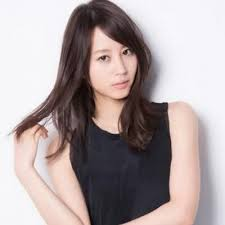
\includegraphics[width=5cm,height=5cm]{index.jpg}
 \end{center}
 \caption{原画像}
\end{figure}

\begin{lstlisting}[basicstyle=\ttfamily\footnotesize, frame=single]
filename = uigetfile('*');
ORG=imread(filename); % 原画像の入力
ORG = rgb2gray(ORG); colormap(gray); colorbar;
imagesc(ORG); axis image; % 画像の表示
pause; % 一時停止
 \end{lstlisting}
を用いてまず入力画像のグレースケール画像を表示させる。

\newpage
\begin{figure}[htbp]
 \begin{center}
  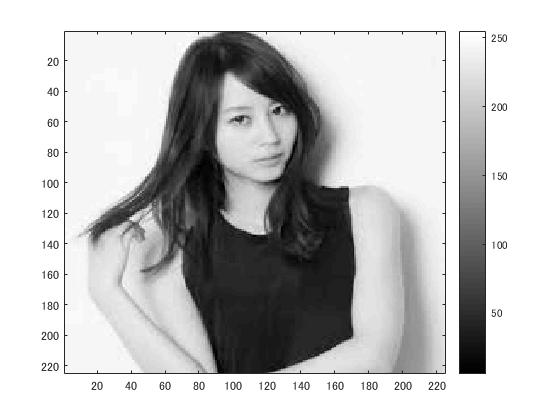
\includegraphics[width=10cm]{kadai5-0.jpg}
 \end{center}
 \caption{グレースケール画像}
\end{figure}

次に
\begin{lstlisting}[basicstyle=\ttfamily\footnotesize, frame=single]
H = imhist(ORG); %ヒストグラムのデータを列ベクトルEに格納
myu_T = mean(H);
max_val = 0;
max_thres = 1;
 \end{lstlisting}
を用いて画像の輝度ヒストグラムを列ベクトルに代入し、全画素の輝度値の中央値を求めて、クラス間分散値/クラス内分散値の最大値、クラス間分散値/クラス内分散値が最大になる
輝度値のしきい値をそれぞれ、0と1で初期化している。また、

\begin{lstlisting}[basicstyle=\ttfamily\footnotesize, frame=single]
for i=1:255
C1 = H(1:i); %ヒストグラムを2つのクラスに分ける
C2 = H(i+1:256);
n1 = sum(C1); %画素数の算出
n2 = sum(C2);
myu1 = mean(C1); %平均値の算出
myu2 = mean(C2);
sigma1 = var(C1); %分散の算出
sigma2 = var(C2);
sigma_w = (n1 *sigma1+n2*sigma2)/(n1+n2); %クラス内分散の算出
sigma_B = (n1 *(myu1-myu_T)^2+n2*(myu2-myu_T)^2)/(n1+n2); %クラス間分散の算出
if max_val<sigma_B/sigma_w
max_val = sigma_B/sigma_w;
max_thres =i;
end;
end;
 \end{lstlisting}
ではしきい値を変化させながら、クラス内の画素数、クラス内平均値、クラス内分散、クラス間分散を算出し、if文内でクラス間分散値/クラス内分散値の最大値とクラス間分散値/クラス内分散値が最大になる輝度値のしきい値を求めている。

\newpage
\begin{figure}[htbp]
 \begin{center}
  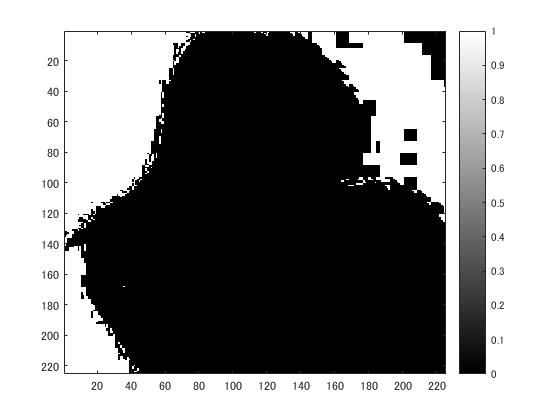
\includegraphics[width=10cm]{kadai5-1.jpg}
 \end{center}
 \caption{判別分析法}
\end{figure}

\section{考察}
今回、判別分析法を用いて画像を変換した、図2と図3を比較すると完璧ではないが背景と人物が2値化により黒色と白色で分けられているのが分かる。

\end{document}